\documentclass[12pt]{article}
\usepackage{amsmath, amssymb, amsthm, amsfonts, geometry}
\newtheorem{theorem}{Theorem}
\newtheorem{lemma}{Lemma}
\newtheorem{proposition}{Proposition}
\newtheorem{corollary}{Corollary}
\newtheorem{definition}{Definition}
\usepackage{tikz}
\usetikzlibrary{automata, positioning}

% Page Setup
\geometry{top=1in, bottom=1in, left=1in, right=1in}

\title{Lecture Notes: Theory of Computation | Introduction (Course: MIT 18.404J)}
\author{Thobias K. Høivik}
\date{\today}

\begin{document}

\maketitle
\section*{Computability Theory vs. Complexity Theory}
\textbf{Computability theory} (prominent 1930s-1950s) is concerned with 
what is computable and not. 
\textbf{Complexity theory} (prominent 1960s-today) is concerned with what is computable 
in practice, and how hard is it to compute a particular problem. 
The first half of this course focuses on \textbf{Computability theory}.  
That means \textbf{Finite automata}, \textbf{Turing machines} and more.

\subsection*{The Role of Theory in Computer Science}  
\begin{enumerate}
    \item Applications 
    \item Basic Research 
    \item Connections to other fields 
    \item What is the nature of computation?
\end{enumerate}

\section*{Finite Automata}
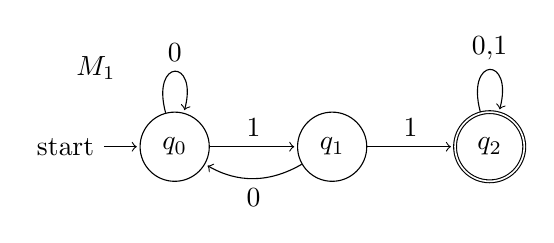
\begin{tikzpicture}[shorten >=1pt, node distance=2cm, on grid, auto] 

   \node[state, initial] (q0)   {$q_0$}; 
   \node[state] (q1) [right=of q0] {$q_1$}; 
   \node[state, accepting] (q2) [right=of q1] {$q_2$}; 

   \node at (-1.0, 1.0) {\(M_1\)};
    \path[->] 
    (q0) edge [loop above] node {0} (q0) 
         edge node {1} (q1)
    (q1) edge node {1} (q2)
         edge [bend left, below] node {0} (q0)
    (q2) edge [loop above] node {0,1} (q2);

\end{tikzpicture}

\noindent 
A \textbf{Finite Automaton} takes a finite string as input and outputs \textbf{accept} 
or \textbf{reject}. The computational process goes as follows: 
\begin{enumerate}
    \item Begin at start state 
    \item Read input symbols 
    \item Follow corresponding transitions 
    \item Accept if end with accept state, Reject if not 
\end{enumerate}

\noindent 
Consider the figure above. Then \(q_2\) is an accepting state. 

\noindent 
\textbf{Examples:}
\[ 
   01101 \to Accept
\]
\[ 
    00101 \to Reject
\]

\noindent 
After some thought we conclude that the strings \(w\) which the automaton \(M_1\), 
seen above, accepts are in \(A\) where \(A = \{w | w \text{ contains substring } 11\}\).
We say that \(A\) is the language of \(M_1\) and that \(M_1\) recognizes 
\(A\) and that \(A = L(M_1)\) (these are three equivalent statements).

\subsection*{Formal Definition} 
\begin{definition}
    A \textbf{finite automaton} \(M\) is a 5-tuple \((Q, \Sigma, \delta, q_0, F)\). 
    \begin{itemize}
        \item \(Q\) finite set of states 
        \item \(\Sigma\) finite set of alphabet symbols 
        \item \(\delta\) transition function \(\delta: Q \times \Sigma \to Q\) 
        \item \(q_0 \in Q\) starting state 
        \item \(F \subseteq Q\) set of accepting states 
    \end{itemize}
\end{definition}

\noindent 
Applying this definition to the automaton \(M_1\) we can formalize as such:  
\begin{gather*}
    M_1 = (Q, \Sigma, \delta, q_0, F) \\ 
    Q = \{q_0, q_1, q_2\} \\ 
    \Sigma = \{0, 1\} \\ 
    F = \{q_3\} \\ 
    \delta = 
    \begin{array}{c|cc}
        \delta & 0 & 1 \\
        \hline
        q_0 & q_0 & q_1 \\ 
        q_1 & q_0 & q_2 \\ 
        q_2 & q_2 & q_2 
    \end{array}
\end{gather*}

\subsection*{String and Languages}
\begin{itemize}
    \item A \textbf{string} is a (usually) finite sequence of symbols in \(\Sigma\). 
    \item A \textbf{language} is a set of strings (finite or infinite).
    \item The \textbf{empty string} \(\epsilon\) is the string of length 0.
    \item The \textbf{empty language} \(\emptyset\) is the set with no strings 
        (i.e the empty set)
\end{itemize}

\noindent 
\textbf{Sidenote:} \(\{\epsilon\} \neq \emptyset\).

\begin{definition}
    \(M\) \textbf{accepts string} \(w = w_1 w_2 \dots 2_n, w_i \in \Sigma\) if there 
    is a sequence of states \(r_0,r_1,r_2,\dots,r_n \in Q\) where: 
    \begin{itemize}
        \item \(r_0 = q_0\)
        \item \(r_i = \delta(r_{i-1}, w_i)\) for \(1 \leq i \leq n\)
        \item \(r_n \in F\)
    \end{itemize}
\end{definition}

\noindent 
The language \(L(M) = \{w | M \text{ accepts } w\}\) is the set of all 
strings accepted by \(M\). We may also write \(L(M)\) is the language of \(M\) or 
M recognizes \(L(M)\).

\begin{definition}[Regular Language]
    A language is regular if some finite automaton recognizes it.  
\end{definition}

\noindent 
Recall \(M_1\): 

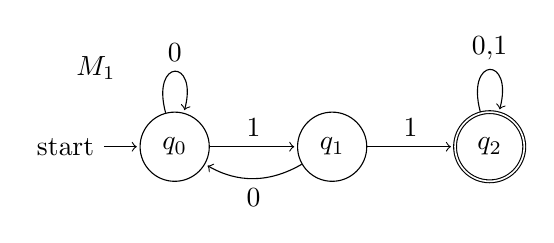
\begin{tikzpicture}[shorten >=1pt, node distance=2cm, on grid, auto] 

   \node[state, initial] (q0)   {$q_0$}; 
   \node[state] (q1) [right=of q0] {$q_1$}; 
   \node[state, accepting] (q2) [right=of q1] {$q_2$}; 

   \node at (-1.0, 1.0) {\(M_1\)};
    \path[->] 
    (q0) edge [loop above] node {0} (q0) 
         edge node {1} (q1)
    (q1) edge node {1} (q2)
         edge [bend left, below] node {0} (q0)
    (q2) edge [loop above] node {0,1} (q2);

\end{tikzpicture}

\noindent 
\(L(M_1) = \{w|w \text{ contains substring } 11\} = A\). 
Therefore \(A\) is regular.

\subsection*{Regular Expressions} 
Let \(A,B\) be languages: 

\noindent 
Union:
\[ 
    A \cup B = \{w|w\in A \lor w\in B\}
\]

\noindent 
Concatenation: 
\[  
    A \circ B = \{xy|x\in A \land y\in B\} = AB
\]

\noindent 
Star: 
\[ 
    A^* = \{x_1\dots x_k | \forall x_i \in A, k \geq 0\}  
\]

\noindent 
\(A^*\) is like the powerset for a language so naturally \(\epsilon \in A^*\) for 
all possible strings \(A\).
Another nice way to write it is 
\[
    A^* = \bigcup_{n=0}^{\infty} A^n
\]
where \(A^n\) is the strings of length n over the language \(A\).

\noindent 
\textbf{Regular expressions} are built from \(\Sigma\), 
members \(\Sigma, \emptyset, \epsilon\) [Atomic], and by using 
\(\cup, \circ, *\) [Composite].

\noindent 
\textbf{Examples: }
\begin{itemize}
    \item \((0\cup 1)^* = \Sigma^* \) gives all strings over \(\Sigma\)
    \item \(\Sigma^* \{1\} = \Sigma^* 1\) gives all strings that end in 1.
    \item \(\Sigma^* 11 \Sigma^*\) gives all strings that contain \(11 = L(M_1)\)
\end{itemize}

\subsection*{Closure Properties for Regular Languages}
\begin{theorem}
    If \(A_1, A_2\) are regular languages, so is \(A_1 \cup A_2\) (closure under \(\cup\)).
\end{theorem}

\begin{proof}
    Let \(M_1 = (Q_1, \Sigma, \delta_1, q_1, F_1)\) recognize \(A_1\)
    and 
    let \(M_2 = (Q_2, \Sigma, \delta_2, q_2, F_2)\) recognize \(A_2\). 
    To show \(A_1 \cup A_2\) to be regular we must construct 
    \(M = (Q, \Sigma, \delta, q_0, F)\) recognizing \(A_1 \cup A_2\). 
    \(M\) should accept input \(w\) if either \(M_1\) or \(M_2\) accept \(w\).

    \noindent 
    We construct \(M\) as follows:
    
    \noindent 
    - The states of \(M\) will be the union of the states of \(M_1\) and \(M_2\), plus a new initial state: 

      \[
      Q = Q_1 \cup Q_2 \cup \{q_0\}
      \]
      where \(q_0\) is the new initial state.
    
      \noindent 
    - The alphabet \(\Sigma\) remains the same as for \(M_1\) and \(M_2\).

    \noindent 
    - The transition function \(\delta\) is defined as follows:
      - For each \(q \in Q_1\), the transitions of \(M_1\) are copied to \(M\):
        \[
        \delta(q, a) = \delta_1(q, a) \quad \text{for all } q \in Q_1, a \in \Sigma.
        \]
      - Similarly, for each \(q \in Q_2\), the transitions of \(M_2\) are copied to \(M\):
        \[
        \delta(q, a) = \delta_2(q, a) \quad \text{for all } q \in Q_2, a \in \Sigma.
        \]
      - Additionally, from the new initial state \(q_0\), we add transitions to the initial states of \(M_1\) and \(M_2\) on \(\epsilon\)-moves:
        \[
        \delta(q_0, \epsilon) = \{q_1, q_2\}
        \]
    
        \noindent 
    - The initial state \(q_0\) is the newly created initial state.

    \noindent 
    - The accepting states \(F\) of \(M\) are the union of the accepting states of \(M_1\) and \(M_2\):
      \[
      F = F_1 \cup F_2
      \]
      This ensures that \(M\) accepts a string if either \(M_1\) or \(M_2\) accepts it.

      \noindent
    Since we have constructed a finite automaton \(M\) that recognizes \(A_1 \cup A_2\), we conclude that \(A_1 \cup A_2\) is a regular language.

\end{proof}

\begin{theorem}
    If \(A_1, A_2\) are regular languages, so is \(A_1A_2\) (closure under \(\circ\))
\end{theorem}
\begin{proof}
    Let \(M_1 = (Q_1, \Sigma, \delta_1, q_1, F_1)\) recognize \(A_1\)
    and 
    let \(M_2 = (Q_2, \Sigma, \delta_2, q_2, F_2)\) recognize \(A_2\). 
    To show that \(A_1A_2\) is regular, we need to construct a finite automaton \(M = (Q, \Sigma, \delta, q_0, F)\) recognizing \(A_1A_2\), the concatenation of \(A_1\) and \(A_2\). 
    We construct \(M\) as follows:

    \noindent 
    - States: The set of states \(Q\) in \(M\) will be the union of the states of \(M_1\) and \(M_2\), along with a new initial state \(q_0\):
      \[
      Q = Q_1 \cup Q_2 \cup \{q_0\}.
      \]
    
      \noindent 
    - Alphabet: The alphabet \(\Sigma\) remains the same as for \(M_1\) and \(M_2\).

    \noindent 
    - Transition function\(\delta\):
      - The transition function for states in \(M_1\) and \(M_2\) will be copied directly from the respective machines:
        \[
        \delta(q, a) = \delta_1(q, a) \quad \text{for all } q \in Q_1, a \in \Sigma
        \]
        and
        \[
        \delta(q, a) = \delta_2(q, a) \quad \text{for all } q \in Q_2, a \in \Sigma.
        \]
      - Additionally, we modify the transitions of \(M\) to connect the final states of \(M_1\) to the initial states of \(M_2\):
        \[
        \delta(f_1, \epsilon) = q_2 \quad \text{for each } f_1 \in F_1.
        \]
        This ensures that after reaching an accepting state of \(M_1\), the automaton can move to the initial state of \(M_2\) without consuming any additional input (via an \(\epsilon\)-transition).

        \noindent 
    - Initial state: The initial state of \(M\) will be the new state \(q_0\), which transitions to the initial state \(q_1\) of \(M_1\) via an \(\epsilon\)-transition:
      \[
      \delta(q_0, \epsilon) = q_1.
      \]

      \noindent 
    - Accepting states: The accepting states of \(M\) will be the accepting states of \(M_2\), because the machine will accept if it reaches an accepting state in \(M_2\) after processing a string in \(A_1\) followed by a string in \(A_2\):
      \[
      F = F_2.
      \]

      \noindent 
    Since we have constructed a finite automaton \(M\) that recognizes \(A_1A_2\), we conclude that the concatenation of \(A_1\) and \(A_2\) is a regular language.

\end{proof}

\end{document}
